\begin{multicols}{2}

\noindent
с длиной волны $\lambda$ определяется групповой скоростью $u = d \omega/dk$ . Групповая скорость u может быть найдена по формуле Эйлера: $u = v - \lambda \frac{dv}{d \lambda}$.
Учитывая, что $v = \omega / k$, из закона дисперсии находим
зависимость фазовой скорости от частоты:
$$ v = \frac{g}{\omega} $$
Из формулы Эйлера для групповой скорости получаем
$$ u = v - \lambda \frac{dv}{d \lambda} = \frac{1}{2}v = \frac{g}{2 \omega} $$
Если расстояние до места падения метеорита $L$, а
регистрация волн началась через время $\tau$ после паде-
ния метеорита, то время прихода групп волн с частотой $\omega = 2 \pi / T$ равна $t' = t + \tau$, т.е.

$$\frac{L}{u} = \frac{L}{g/(2\omega)} = t + \tau \textrm{, или } \omega = \frac{g(t + \tau)}{2L}$$

Получается, что частота $\omega$ линейно растет со временем, причем угловой коэффициент прямой $\omega(t)$ равен $A = g/(2L)$. Построим график зависимости $\omega = \omega(t)$, соответствующий таблице 2.

\null\hfill \textit{Таблица 2  }

\noindent
\scalebox{0.7}
{
\begin{left}
\begin{tabular}{|c|c|c|c|c|c|c|c|c|c|c|}
\hline
     t, ч & 0 & 3 & 6 & 9 & 12 & 15 & 18 & 21 & 24 & 27 &
 \hline
     $\omega, c^-1$ & 1,10 & 1,26 & 1,46 & 1,70 & 1,90 & 2,02 & 2,24 & 2,4 & 2,5 & 2,73 &
 \hline
\end{tabular}
\end{left}
}

\columnbreak

\begin{Figure}
 \centering
 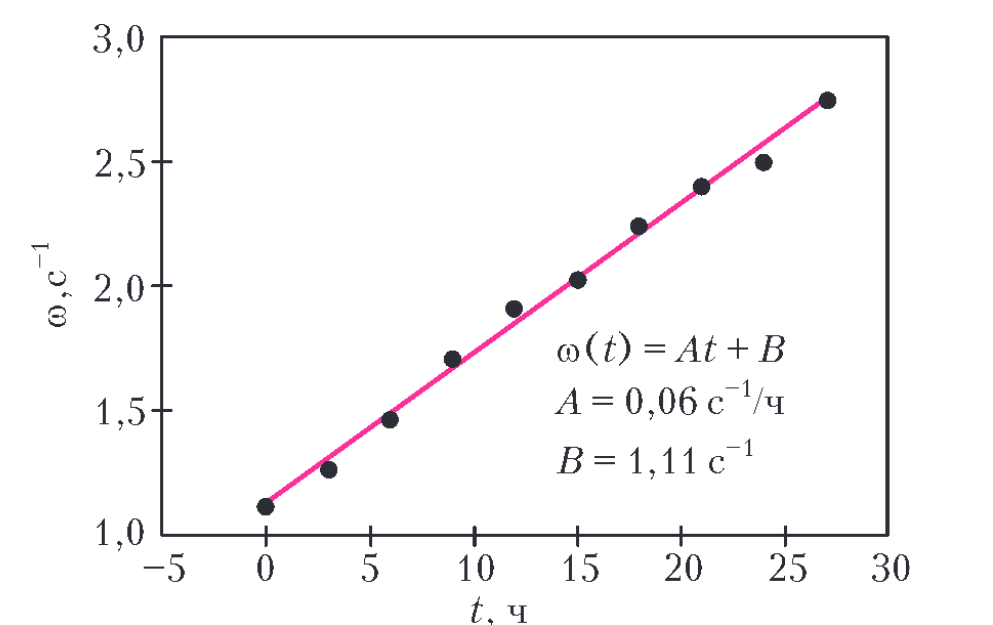
\includegraphics[width=\linewidth]{sc.png}
 \captionof{figure}{my caption of the figure}
\end{Figure}

График, приведенный на рисунке, хорошо описывается прямой $\omega(t) = At + B$ с угловым коэффициентом 
$$A = \frac{\Delta \omega}{\Delta t} = 0,06 \textrm{ c}^{-1}/\textrm{ч}.$$
Отсюда находим расстояние до места падения спутника на землю:
$$L = \frac{g}{2A} \approx 300 \textrm{км.}$$

Метеорит упал за $\tau = B/A = 18,5$ ч до начала наблюдений. Учитывая, что наблюдения за волнением начались в 12:00, момент падения метеорита соответствует времени 17:30 предшествующих дню наблюдения суток.

\end{multicols}

\begin{box}
  \centering
  \tcbox[top=10pt,left=150pt,right=150pt,bottom=0pt, colback=orange!50, colframe=orange!50!orange!50]{\large\textbf{НАМ ПИШУТ}\normalsize}
\end{box}

\begin{multicols}{2}
{
\centering
\Large
  \centering \textbf{Глиняные гири}
\normalsize
\par
}

Не секрет, что математика – вовсе не сухая и скучная наука. В ней много интересных задач, и бывает, что впечатление от решения красивой задачи запоминается на всю жизнь.
О таком ярком моменте из своих школьных лет написал нам наш читатель из города Пересвет Московской области Данил Владимирович Поташников, ветеран Великой отечественной войны. Вот несколько его строк о себе:

«В 1961 году закончил МАИ очно. В 1999 году заочно освоил пятигодичный курс Открытого университета Израиля. Не пропустил ни одну лекцию из цикла «Академиятелеканала «Культура».

А вот выдержка из его письма о запомнившейся задаче:
«Когда я учился в пятом классе (а это было в городе Каменка Черкасской области на Украине в 1936 году), учитель математики записал на доске домашнее задание и попросил дополнительно решить головоломку.

На Украине в XIX веке гири для рычажных весов изготавливались и самодельные – из глины. Самая большая была пудовая (40 фунтов). По дороге на ярмарку пудовая гиря упала с воза и разбилась на четыре части. Оказалось, что этими частями можно взвесить на рычажных весах любые покупки весом от одного до сорока фунтов. Суть задания: найти вес каждой части.

Никогда не забуду ту бессонную ночь!

\columnbreak
Когда я назвал вес каждой части: 1, 3, 9, 27, учитель попросил выйти к доске и пояснить ответ.

Один фунт – нелогично использовать две части для определения одного фунта.

Три фунта – «1» и «3» позволят взвесить 1, 2, 3 и 4 фунта.

Девять фунтов – сможем взвесить от 5 до 13 фунтов.

Двадцать семь фунтов – сможем взвесить от 14 до 40 фунтов.
На одной из последних встреч с учениками 6-го класса я попросил решить эту головоломку. Я сообщил детям свой телефон и обещал подарок тому, кто первый найдет решение.

Увы!»

Предлагаем нашим читателям справиться с таким обобщением этой головоломки, ставшим классической олимпиадной задачей: \textit{Докажите, что с помощью n гирь массами $1, 3, 9, \dots, 3^{n - 1}$ кг можно взвесить на чашечных весах любой предмет массой $M \leq \frac{3^n - 1}{2}$ кг (M - целое число, гири можно класть на обе чаши весов).}

В завершение приведем еще одну цитату из письма
Д.В.Поташникова:

«В этом году по просьбе детей и внуков я написал свои воспоминания, которые закончил словами «Я живу, пока познаю».
\end{multicols}
